在汽车领域有许多
威胁分析和风险评估(TARA)方法。SAE J3061
\cite{sae2016cybersecurity}作为
第一本针对网络物理车辆系统的网络安全指南,提出了
EVITA(电子安全车辆入侵保护应用程序)、HEAVENS (修复漏
洞以增强软件安全性)、TVRA(威胁、漏洞和风险分
析)、OCTAVE(运营关键威胁、资产和漏洞评估)以及其
他安全分析方法。然而,并不是所有提到的方法都适用
于智能网联汽车。TVRA是为数据和电信网络开发的,
不适用于汽车。OCTAVE适用于企业信息安全的风险评
估,但不适用于汽车系统。只有EVITA和HEAVES更适合智能汽
车领域。

\subsection{车载内部网络通信技术}
现代车载通信系统中有五种最广泛使用的车载网络:LIN(本地互连网络)、CAN(控制器局域网)、FlexRay、以太网和 MOST(面向媒体的系统传输)。各有优势和劣势。
根据实际观察,LIN 经常用于通常不需要严格时序性能的低速通信。CAN 广泛部署在动力总成和车身控制领域,也是从车辆中检索 OBD(车载诊断)数据的标准接口。
FlexRay 具有高确定性和容错性,
这通常在高级底盘控制和通信主干等应用中需要。有线以太网在量产汽车中仍然相对较新,可能仅用于 ECU 闪烁和有限的网络主干连接等应用。
然而,它在延迟和抖动非常有限的高速数据传输方面具有巨大潜力。因此,以太网在未来可能会获得更多车载网络的份额。

\begin{itemize}
    \item LIN 是一种低成本、低速且易于实现的车载网络,主要用于简单且时间要求不高的应用,例如传统的中央门锁激活、车窗升降器控制、后视镜调节,方向盘按钮模块,以及许多低刷新率传感器。LIN 最突出的优势是它的成本比其他主要网络低得多[18]. 这种优势来自多个方面。首先,LIN控制器相对便宜。LIN 模块使用 UART(通用异步接收器/发送器)端口来发送和接收串行数据。
    \item CAN网络长期以来一直用于传输大部分车载通信信号。尽管后来针对 CAN 无法满足的一些要求开发了各种不同的网络,但 CAN 在汽车网络中仍然保持着普及,特别是在动力总成系统和上半身电子设备中。车辆中的 CAN 芯片估计数量已接近 5 亿个。最近的一项预测甚至预计 CAN 网络将在未来十年内继续在车载通信系统中蓬勃发展。
    \item 出于解决不确定性、增加带宽和增强 LIN 和 CAN 等网络的抗故障能力的目标,FlexRay 由 FlexRay 联盟发起。目前,它已越来越多地应用于车辆动力学领域和域间通信。FlexRay 网络比 LIN 和 CAN 具有更快的传输速度和更高的容错性。它的成本也明显更高,尽管 FlexRay 系统的实际成本可能存在争议。FlexRay 的传输能力有三个最突出的特性: 1) 它可以在同一周期内传输确定性和动态数据;2)它比LIN和CAN(包括TTCAN和CANFD)具有更大的有效载荷;3)在网络拓扑方面非常灵活。
    \item 随着在新型车辆中越来越多地实施 ADAS 和多媒体功能,强烈要求更宽的车辆网络带宽。以太网是超越 CAN 和 FlexRay 的下一代车载网络的一个非常有前途的候选者。近年来,它越来越受到汽车行业的关注。到 2023 年,以太网在新车中的渗透率将高达 40\%。
\end{itemize}

由于现代车载通信系统几乎总是由运行不同通信协议的各种子网组合而成,因此作为不同子网之间接口的汽车网关对于整个车载通信网络至关重要,不容忽视。

通信系统中的汽车网关通常具有三种可能的功能。首先,它可以作为一个协议桥来促进跨不同子网的数据传输。这也是网关最正统的作用。其次,它可以用来“扩展”网络带宽,网关连接到相同协议的其他子网,以避免一个网段过载。第三,网关可以作为防火墙工作,在其中它起到保护作用,以抵御未经授权的外部访问尝试并最大程度地减少不希望的干扰。

网关有两种分类。如果基于路由机制,网关可以分为消息路由或信号路由。如果根据ECU的整体功能,网关可以分为独立的或集成的。

消息路由网关通常根据路由表将入口消息路由到指定的子网,有时甚至不改变传入消息的 ID 或传输周期(例如,路由到相同协议但具有不同协议的网络)波特率)。参考 OSI 模型,只需要到网络层的功能来完成消息路由。相反,信号路由网关需要解包入口消息,重构新消息,并将它们发送到指定的子网。通常,信号路由网关比消息路由网关的计算要求更高,并且可能需要在 OSI 模型方面实现高于网络层的软件。不同协议之间的网关(例如 CAN 和 FlexRay 之间,

另一方面,独立网关是仅用于路由而没有任何其他应用功能(通常除了网络管理和诊断)的网关。集成网关不仅可以路由消息,还可以部分作为具有其他功能的普通 ECU,例如车身控制或插图面板控制。

在车载网络设计中,独立网关和集成网关之间的选择主要取决于 ECU 的成本和计算能力。集成网关更便宜,但需要更多的计算能力,因为它们还需要同时完成非路由任务。独立网关可能会带来额外的硬件成本,例如新的 ECU 和电线,但可以在系统设计、组件测试、维护甚至封装方面带来极大的灵活性和便利性。

在为实际应用设计汽车网络网关时,过程变得更加复杂,并且可能因情况而异。在高度分布式的车载网络中,如何应对网络复杂性不断提高、域间通信量大、时序要求严格、带宽需求增加等挑战,已成为当今汽车网关研究的热门话题。此外,网关的软件架构也非常关键。由于网关在汽车中非常灵活,因此其软件也应该非常易于实施,并满足未来开发的可靠性、可维护性、可重用性和可移植性等质量要求。


攻
击树模型是 Schneier Bruce 在上世纪末提出的一种威胁建模方法\cite{schneier1999attack},其年代久远,
理论也日益完善。此方法使用树形结构搭建攻击模型,让建模人员从面临黑客攻击
的角度考虑问题,树形结构的每一个节点,都必须被慎重考虑和布局,因为每个节
点的配置稍有不慎,都有可能被黑客攻击。攻击树模型的优点是可以利用简单的网
络模型构建复杂的威胁类型和攻击方式,其扩展性强。这样的结构,还可以从深度
优先和广度优先不同的策略来考虑问题。当整个攻击树模型足够完整时,就可以很
好的预防威胁,抵御非法攻击。不过,其劣势也非常明显,由于攻击树模型完全是
从黑客的角度来思考问题的,因而,建模者必须要具备很强的技术能力,并且有较
好的攻击经验,所以难易大规模实施基于攻击树模型的威胁建模。


\subsection{CVSS模型}

通用漏洞评分系统(CVSS)(2007 年完成,第 2 版)被认为是衡量软件漏洞相对严重性的规范,可应用于大
量系统,包括那些属于美国联邦机构的系统\cite{mell2007common}。
CVSS 由三个不同的度量组组成:基础、时间和环境。每一个都由它们自己的一套度量标
准组成。基本度量组可用于大多数情况,但也可以将其他值分配给其他度量组,以便为特定漏洞提供额
外的上下文。这些度量组可以描述如下:
\begin{itemize}
    \item  基础表示漏洞的特征,这些特征会随着时间和用户环境的变化而不断变化
    \item  时态表示漏洞随时间变化的特征,但不提及用户环境
    \item  环境表示与用户的特定环境相关和/或独特的漏洞特征
\end{itemize}

一旦为这些基本指标中的每一个分配了一个值,基本公式就会计算出一个范围从 0 到 10 的分数。根据所
有因素,从等式中创建一个向量,并将该向量输出为包含分配给每个指标的值的文本字符串,以便准确
传达如何为每个发现的漏洞得出分数。该过程如图 2.8 所示。
\begin{figure}
    \centering
    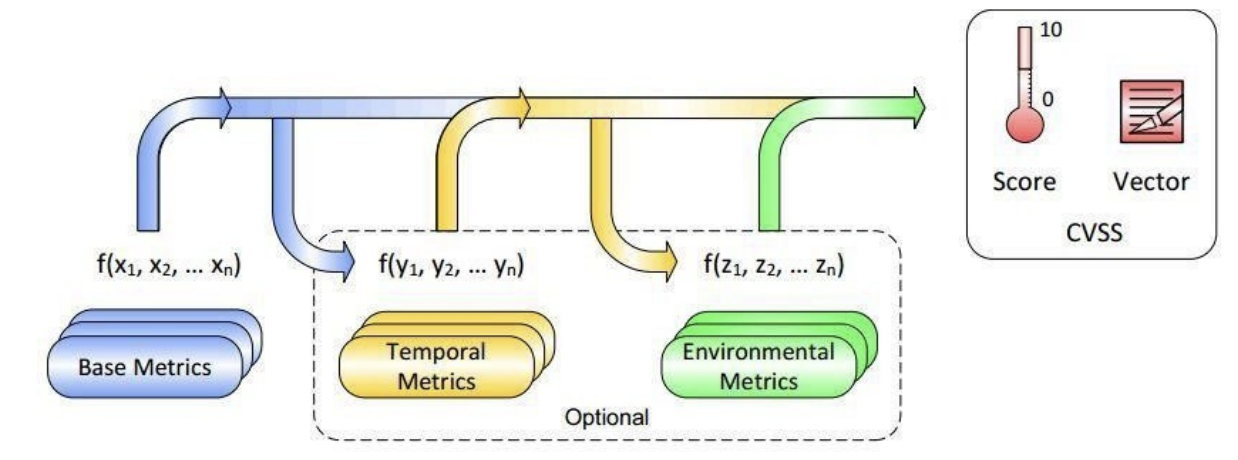
\includegraphics[scale=0.6]{resources/img/i9.png}
    \caption{CVSS的度量和方程组合起来创建矢量}
  \end{figure}

  \subsection{HEAVENS安全模型}
  如图2.9所示,HEAVENS安全模型\cite{haringajoint}旨在识别所有者、资产、风险、漏洞、对策、威胁代理和威胁,并将所有方面
整合在一起,以建立汽车行业的安全模型。此外,我们的目标是在汽车电子/电子系统的背景下研究来
自其他领域(例如,IT 安全、电信和国防)的安全模型。因此,在HEAVENS安全模型中,第一步是从涉众(即
所有者)的角度识别用例。用例随后被用于识别资产和威
胁,包括可能受到特定威胁影响的安全属性。在风险评估期间,威胁代理(攻击者)的角色以及攻击对特
定资产的影响已被考虑,以对威胁进行评级,即识别风险。这有助于确定安全要求和可能的对策,以解
决特定资产的特定威胁。

\begin{figure}
    \centering
    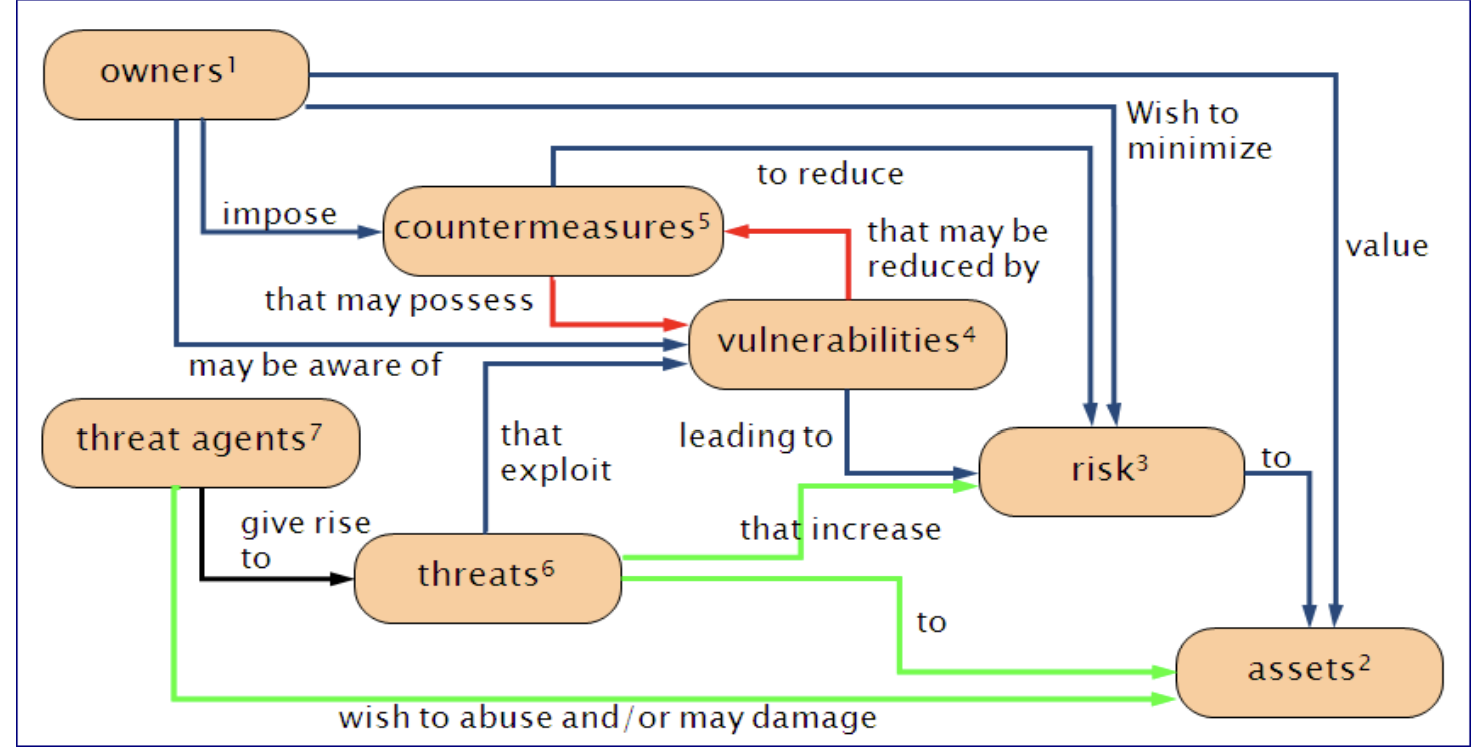
\includegraphics[scale=0.6]{resources/img/i10.png}
    \caption{典型的威胁风险评估图}
  \end{figure}

  HEAVENS安全模式的优势如下:

  \begin{itemize}
    \item  所提出的模型同样适用于各种道路车辆,例如客车和商用车。该模型考虑了广泛的利益相关方 (例
    如,原始设备制造商、车队所有者、车主、驾驶员、乘客等)。
    \item  时通过在汽车电子电气系统环境中应用微软的 STRIDE 方法实现的以威胁为中心的模型。它通过仅使用
    少数通用威胁类别,而不是考虑与资产相关的几乎无限的攻击可能性和攻击技术,来支持更好地理
    解可能的攻击的影响。
    \item  该模型在威胁分析期间建立了安全属性和威胁之间的直接映射。这有助于对特定资产的特定威胁的
    技术影响(机密性、完整性、可用性)进行可视化和早期评估。
    \item 该模型将安全目标(安全、财务、运营、隐私和法规)与风险评估期间的影响级别估计对应起来。这
    有助于了解特定威胁对相关利益方(例如 OEM)的潜在业务影响。
    \item 该模型符合成熟的行业标准和计划。例如,通用标准ISO-26262。这有助于
    重用其他研究领域已经存在的过程,例如,功能安全。它还提供了一个了解跨安全和安保领域的网
    络安全问题的机会。
\end{itemize}

HEAVENS安全模型的主要目标是推导出TOE的安全要求,即TOE的资产,类似于ISO-26262中所述的功能安全要求的概念。
为了实现这一点,我们为与构成 TOE 的资产相关的每个已识别的
威胁建立了一个安全级别。因此,HEAVENS安全模型包括威胁分析和风险评估。因此,“HEAVENS安全模型”指
的是威胁分析和风险评估,以便通过应用HEAVENS方法和工具支持来推导特定 TOE 的安全要求。
图 2.10 显示了HEAVENS安全模型的工作流程。它由三部分组成——威胁分析、风险评估和安全要求。
HEAVENS安全模型的工作流程如下:
\begin{itemize}
    \item  威胁分析–功能用例的描述(图中的 In\_01)是威胁分析流程的输入。威胁分析产生两个输出:(a)用例环境中每个资产的威胁和资产之间的映射(图中的Out\_01),
    以及(b)威胁和安全属性之间的映射(图中的Out\_02),以确定哪些安全属性由于资产环境中的特定威胁而受到影响。
    \item  风险评估—一旦确定了相关资产的威胁,下一步就是对威胁进行分级。这是在风险评估期间完成的。威胁和资产之间的映射与威胁级别(TL)(图中的 In\_03)和影响级别(IL)
    (图中的 In\_04)参数一起用作输入。作为风险评估的最终结果,我们为与TOE/用例的每个资产相关联的每个威胁确定安全级别(图中的 Out\_03)。
    \item  安全要求–最后,我们考虑威胁和资产之间的映射(图中的 Out\_02 是威胁分析的结果)以及安全级别(图中的 Out\_03 是风险评估的结果)来制定资产和 TOE 的安全要求。
    安全需求是资产、威胁、安全级别和安全属性的函数。请注意,安全级别根据与特定资产相关联的特定威胁的安全目标来考虑潜在的业务影响。
    衍生的安全要求处于 ISO-26262 功能安全要求的水平,属于概念阶段。之后,在产品开发阶段,需要根据高级安全需求派生出软件安全需求和硬件安全需求。
  \end{itemize}


\begin{figure}
    \centering
    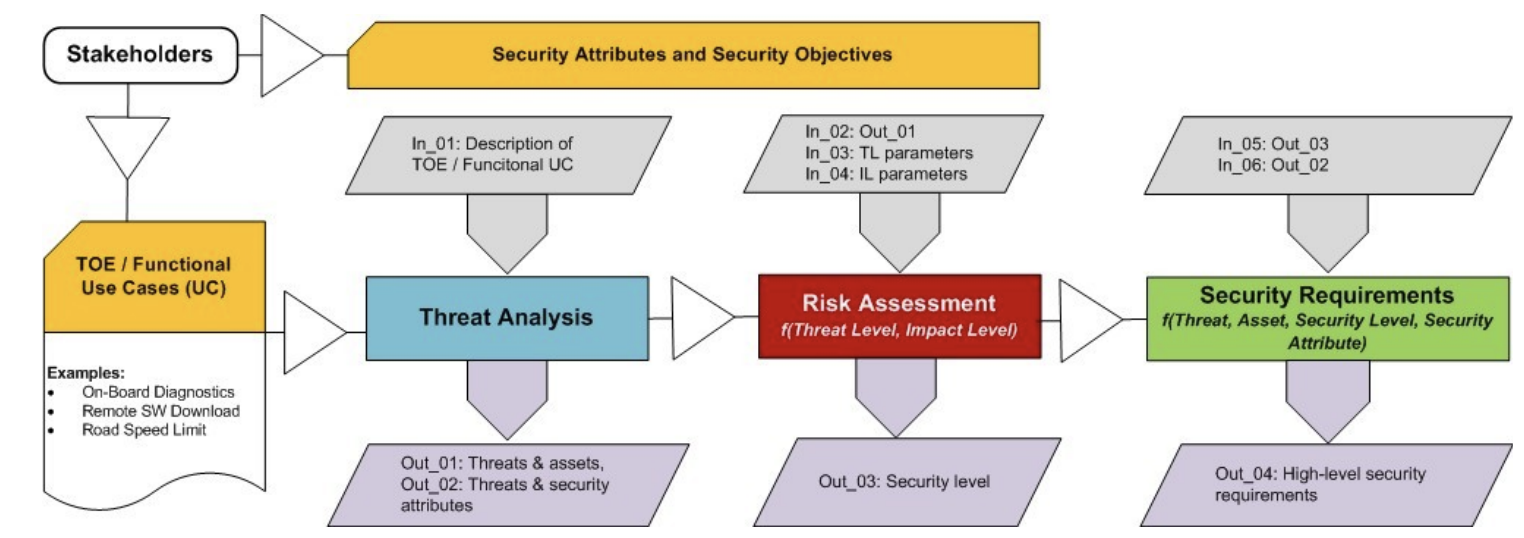
\includegraphics[scale=0.6]{resources/img/i11.png}
    \caption{HEAVENS安全模型工作流程图}
  \end{figure}


  \section{威胁建模步骤}
要进行有效的威胁建模,首先需要以下利益相关者的意见:
  \begin{itemize}
    \item 提供应用程序的业务影响的业务利益相关者。
    \item 架构师提供应用生态系统的概述。
    \item 用于特定代码输入的程序员,例如使用的框架、编码指南等。
    \item DevOps提供服务器和网络配置的详细信息。
    \item 专家学者在关键参数上的影响因子
  \end{itemize}
  其次是威胁建模的具体步骤,图3.1是威胁建模的步骤图:
  \begin{itemize}
    \item 设计:明确系统的所有要求,并创建数据流关系图。
    \item 中断: 将威胁建模框架应用到数据流关系图,并查找潜在的安全问题。
    \item 修复: 确定如何正确组合安全控制来解决每个问题。
    \item 验证: 验证是否满足了要求、找到了问题并实现了安全控制。
  \end{itemize}
  \begin{figure}
    \centering
    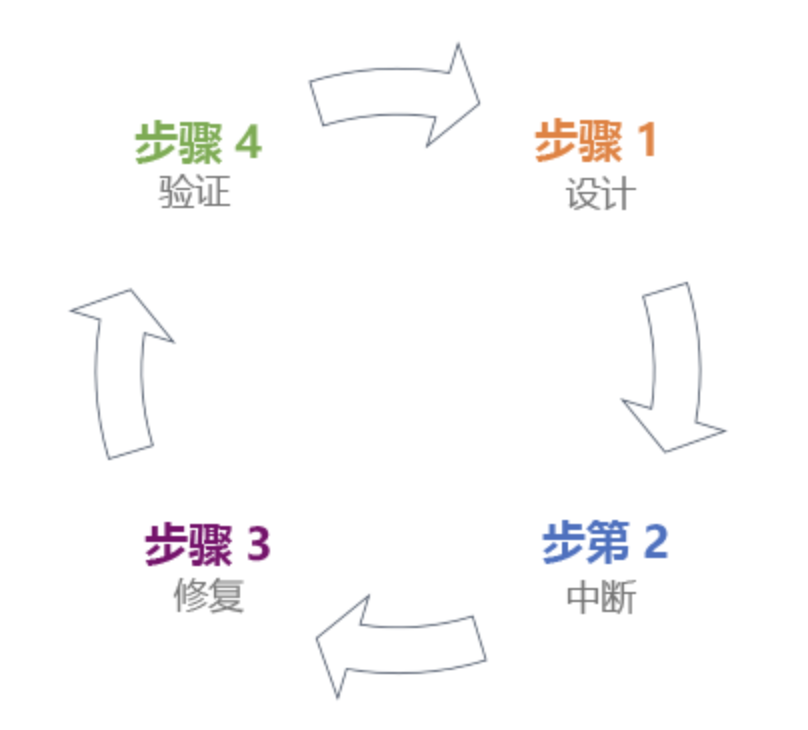
\includegraphics[scale=0.6]{resources/img/i4.png}
    \caption{威胁建模步骤}
  \end{figure}

\subsection{设计}
设计阶段是进行威胁建模活动的基础。 你需要尽可能多地收集关于你所构建的内容及所用资源的数据。
清楚地了解系统的工作原理,列出系统使用的每个服务,枚举有关环境和默认安全配置的所有假设,使用正确的上下文深度级别创建数据流关系图。
尽可能多地提出有关系统的问题。 可以考虑以下问题:
保护数据免受未经授权的披露的机密性。
防止未经授权的信息更改的完整性。
即使系统受到攻击也能提供所需的服务。
系统如何处理密钥、证书和凭据?
需要保护哪些商业秘密和知识产权?
想在威胁建模上花费多少时间和金钱?
\newline
在设计阶段"可视化"是非常重要的步骤.对整个应用程序的清晰记录的概述将大大简化流程。这包括记下用例、数据流、数据模式和部署图。您可以构建两种类型的可视化。
数据流图:它描述了数据是如何设计为在您的系统中移动的。它显示了操作级别,并清楚地显示了数据进入和退出每个组件的位置、数据存储、流程、交互和信任边界。 
流程图:它描述了用户如何在各种用例中交互和移动。它处于应用程序级别。DFD 专注于系统内部的工作方式,而 PFD 则专注于用户和第三方与系统的交互。您可以选择其中之一或同时使用两者。
这里介绍下创建数据流关系图: 数据流关系图是系统的图形表示形式,应指定每个元素及其交互和上下文。
数据流关系图显示了给定系统中的数据流。 它通常以用户或数据存储的请求开始,以数据存储或 Analytics Services 结束。 数据流关系图使用不同的形状来指示它们所表示的元素。
如元素:过程一般用圆形来表示,其定义:接收、修改输入或将输入重定向到输出的任务,如 Web 服务。
外部实体用矩形来表示,其定义:直接控制之外的任务、实体或数据存储,如用户和第三方 API。
数据存储一般用形如"二"汉字来表示,其定义:永久和临时数据存储,如 Web 缓存和 Azure 托管数据库。
数据流关系图应当包含:正在构建的系统类型和安全团队所需的上下文。	

\subsection{中断}
在中断阶段,需使用数据流关系图查找针对系统的潜在威胁。 此过程使用威胁建模框架,以帮助你查找最常见的威胁和防范威胁的方法。
选择以“保护系统”或“了解攻击者”为核心的方法, 如使用微软的STIRIDE威胁模型识别常见威胁。
选择重点领域和相关框架,以系统地识别系统中的潜在威胁。

\subsection{修复}

在修复阶段,需要决定如何处理所有威胁。 比如每个STRIDE威胁都对应到一项或多项安全控制,这些控制措施提供不同的功能和类型供你选择。
并且获得与每个资产及其操作相关的威胁的主列表或库以及可能的攻击者配置文件列表。
具体来讲:该阶段目标如下:
\begin{itemize}
    \item 根据优先级框架或安全 bug 栏衡量每个威胁的优先级
    \item 将每个威胁作为任务或工作项进行跟踪
    \item 生成对应于 STRIDE 威胁的安全控制建议
    \item 选择一项或多项安全控制类型和功能来应对每个威胁
    \item 解决任务
  \end{itemize}

\subsection{验证}

验证阶段是威胁建模过程的最后一步,通常发生在部署系统之前。 它涉及到确保满足要求、验证假设以及准备好安全控制。
确认系统满足所有新旧安全要求,配置云提供商、操作系统和组件以满足安全要求,确保使用正确的安全控制解决所有问题,在部署前对系统进行手动和自动验证。
在验证期间,需要我们检查是否所有漏洞都已得到解决。并自问以下问题:所有的威胁都被缓解了吗?是否清楚地记录了剩余风险?
完成此操作后,需要决定管理已识别威胁的后续步骤,并决定下一次威胁建模迭代的时间。
威胁建模不是一次性活动。它需要在预定的时间间隔或在应用程序开发的特定里程碑期间重复。

